\chapter{CƠ SỞ LÝ THUYẾT VÀ CÔNG TRÌNH LIÊN QUAN}
\label{chap:chap2-theory}

Trong chương này, tác giả trình bày cơ sở lý thuyết nền tảng cho bài toán Hỏi–đáp hình ảnh (Visual Question Answering -- VQA), các kiến trúc học sâu liên quan (CNN, RNN/LSTM, Transformer và các module attention), đồng thời tập trung phân tích mô hình CLIP — một mô hình đa phương thức học đối sánh ảnh-văn bản. 
Chương cũng tổng hợp các công trình nghiên cứu quan trọng liên quan tới VQA nói chung và VQA trên dataset VizWiz nói riêng, kết luận bằng việc khảo sát những thách thức còn tồn tại và các hướng nghiên cứu tiềm năng.

\section{Bài toán VQA}
Bài toán VQA đặt vấn đề: với một cặp (hình ảnh, câu hỏi bằng ngôn ngữ tự nhiên), mô hình cần sinh ra một câu trả lời ngắn gọn (thường là một từ, cụm từ ngắn hoặc câu). VQA là bài toán đa phương thức (multimodal) kết hợp thị giác máy tính và xử lý ngôn ngữ tự nhiên, đòi hỏi mô hình phải:
\begin{itemize}
    \item Trích xuất biểu diễn thị giác giàu thông tin từ ảnh.
    \item Mã hoá nội dung ngôn ngữ của câu hỏi.
    \item Kết hợp hai miền biểu diễn để suy luận và chọn câu trả lời.
\end{itemize}

\section{Đặc điểm của dataset VizWiz}
Dataset \textbf{VizWiz} được thu thập từ người dùng khiếm thị: họ chụp ảnh bằng điện thoại và ghi câu hỏi bằng giọng nói. Những điểm cần lưu ý của VizWiz:
\begin{itemize}
    \item Quy mô: hơn 31.000 cặp (ảnh, câu hỏi) với nhiều đáp án crowdsourced cho mỗi câu hỏi.
    \item Chất lượng ảnh thường kém: mờ, bị che khuất, framing sai, ánh sáng xấu — do ảnh được chụp bởi người khiếm thị. 
    \item Câu hỏi mang tính hội thoại, tự nhiên, và có tỉ lệ lớn các câu hỏi \textbf{không thể trả lời} (unanswerable) do ảnh thiếu thông tin.
    \item Tập dữ liệu đặt ra hai nhiệm vụ: (1) trả lời câu hỏi; (2) xác định một câu hỏi có thể trả lời từ ảnh hay không (answerability).
\end{itemize}

\section{Các kiến trúc học sâu liên quan trong VQA}
Dưới đây là các thành phần/kiến trúc thường gặp trong pipeline VQA.

\subsection{Trích xuất đặc trưng hình ảnh (CNN / backbone)}
Mạng tích chập như VGG, ResNet, EfficientNet hay các biến thể ViT/CNN hiện đại được dùng để sinh feature maps hoặc region features (ví dụ object proposals / Faster R-CNN) làm đầu vào cho phần hợp nhất (fusion).\\

\subsection{Mã hoá câu hỏi (RNN / Transformer)}
Trước đây phổ biến dùng LSTM/GRU để mã hoá câu hỏi; hiện nay Transformer (hoặc BERT-like encoder) được ưa chuộng hơn vì khả năng mô hình hóa tương tác từ xa và đạt hiệu năng tốt trên các embedding ngôn ngữ.\\

\subsection{Cơ chế Attention và Fusion}
Một bước quan trọng là cho phép mô hình “chú ý” tới vùng ảnh có liên quan tới từng từ/cụm từ trong câu hỏi. Các cơ chế attention (Stacked Attention Network, Bilinear Attention, Co-attention) và các phương pháp fusion (concatenation, bilinear pooling, multimodal transformer) là lõi của nhiều mô hình VQA thành công.

\subsection{Các kiến trúc đa phương thức hiện đại}
Các mô hình dựa trên transformer đa phương thức (ví dụ ViLBERT, LXMERT, VisualBERT, UNITER...) kết hợp encoder cho ảnh và text, hoặc dùng mô hình tự hồi tiếp (cross-attention) để tương tác giữa hai luồng đại diện. Những mô hình này thường fine-tune lên tập VQA để đạt hiệu quả cao.

\section{Mô hình CLIP: nguyên lý và vai trò trong VQA}
\subsection{Nguyên lý hoạt động}
CLIP (Contrastive Language–Image Pretraining) học đồng thời hai encoder: một encoder ảnh và một encoder văn bản. Mục tiêu huấn luyện là tối đa hóa độ tương đồng (cosine similarity) giữa embedding của ảnh và embedding của caption tương ứng, và giảm độ tương đồng với các cặp không tương ứng thông qua bài toán contrastive learning. Sau khi huấn luyện, ảnh và văn bản nằm trong cùng một không gian embedding, cho phép:
\begin{itemize}
    \item So sánh trực tiếp ảnh với các mô tả văn bản (text prompts).
    \item Thực hiện \emph{zero-shot classification} bằng cách so sánh ảnh với các prompt mô tả nhãn.
\end{itemize}

\begin{figure}[!hbt]
    \centering
    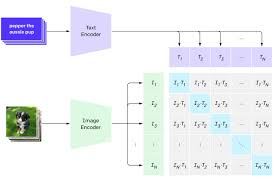
\includegraphics[width=1.0\linewidth]{graphics/chapter2/CLIP_model.jpg}
    \caption{Hình ảnh minh họa nguyên lý hoạt động của CLIP}
\end{figure}
\subsection{Ưu điểm khi áp dụng cho VQA}
\begin{itemize}
    \item \textbf{Tổng quát hóa tốt:} CLIP được huấn luyện trên hàng trăm triệu cặp ảnh-văn bản nên có kiến thức ngữ nghĩa rộng.
    \item \textbf{Zero-shot / Few-shot:} CLIP có thể áp dụng trực tiếp cho các nhãn mới bằng prompt, thuận lợi cho các bài toán có nhãn phong phú hoặc hiếm.
    \item \textbf{Linh hoạt trong thiết kế pipeline:} CLIP có thể dùng làm backbone trích xuất embedding ảnh và/hoặc encoding câu trả lời/câu hỏi bằng text encoder.
\end{itemize}

\subsection{Chiến lược ứng dụng CLIP cho VQA}
Một số chiến lược phổ biến:
\begin{itemize}
    \item \textbf{Zero-shot VQA:} Tạo tập các câu trả lời ứng viên (ví dụ top-K answers) thành các prompt (ví dụ "A photo of a \{answer\}") rồi so sánh embedding câu hỏi+ảnh với embedding prompt, chọn đáp án có độ tương đồng cao nhất.
    \item \textbf{Fine-tune hoặc thêm head:} Giữ encoder CLIP cố định hoặc tinh chỉnh, thêm một lớp phân loại (linear head) hoặc module cross-attention để tối ưu hoá cho VQA.
    \item \textbf{Kết hợp với mô-đun reasoning:} Dùng CLIP để lấy embedding ban đầu, sau đó áp dụng mô hình cross-modal transformer hay module reasoning để giải các câu hỏi đòi hỏi suy luận phức tạp.
\end{itemize}

\section{Tổng hợp các công trình liên quan (tập trung VizWiz)}
\subsection{Nghiên cứu nền tảng về VizWiz}
Dataset và bài toán VizWiz được giới thiệu để khuyến khích nghiên cứu hỗ trợ người khiếm thị trong môi trường thực; tác giả gốc phân tích rằng các thuật toán VQA cổ điển gặp khó trên VizWiz do chất lượng ảnh và tính answerability. (\emph{Nguồn cơ sở: bài báo giới thiệu VizWiz và trang chính thức của dự án}.)\nocite{Gurari2018}

\subsection{Các phương pháp truyền thống áp dụng cho VizWiz}
Trong nhiệm vụ VizWiz Grand Challenge (CVPR/ECCV), nhiều đội thi áp dụng kiến trúc kết hợp CNN + LSTM/attention (ví dụ: mô hình sử dụng Faster R-CNN để lấy region features kết hợp Bilinear Attention Network), và bổ sung bộ phân loại để phát hiện câu hỏi không thể trả lời. Những cải tiến tập trung vào:
\begin{itemize}
    \item Xử lý ảnh đầu vào: tăng cường (augmentation), loại bỏ vùng nhiễu, hoặc áp dụng super-resolution/denoising trước khi trích xuất feature.
    \item Module xác định answerability (binary classifier) tách biệt.
    \item Fine-tuning trên VizWiz và sử dụng ensemble để cải thiện độ chính xác.
\end{itemize}

\subsection{Các công trình gần đây và xu hướng sử dụng CLIP}
Trong những năm gần đây, CLIP được sử dụng như một backbone đa phương thức cho nhiều tác vụ, bao gồm VQA. Các nghiên cứu cho thấy chiến lược fine-tune CLIP hoặc sử dụng CLIP cho zero-shot/few-shot có thể đem lại cải thiện, nhưng vẫn cần module reasoning hoặc cross-attention để xử lý các câu hỏi yêu cầu suy luận hoặc tri thức ngoài ảnh. (\emph{Một số công trình thực nghiệm đã áp dụng CLIP cho VQA với việc thêm linear head hoặc mô-đun cross-modal.})

\section{Đánh giá hiệu năng và metrics cho VizWiz}
Các metric thường dùng trong VQA:
\begin{itemize}
    \item \textbf{Accuracy} (đặc biệt cho các câu trả lời ngắn như Yes/No).
    \item \textbf{VQA accuracy} (tính toán trên nhiều người anotate — điểm trung bình có trọng số).
    \item \textbf{Precision/Recall/F1} cho task phân biệt answerable/unanswerable.
\end{itemize}
Khi làm việc với VizWiz cần cân nhắc: phân bố nhãn bị lệch, nhiều đáp án không đồng nhất (crowdsourced), và ảnh chất lượng thấp làm giảm độ tin cậy của metric đơn giản.

\section{Những thách thức đặc thù của VQA trên VizWiz}
\begin{enumerate}
    \item \textbf{Chất lượng ảnh và framing không chuẩn:} ảnh bị mờ, bị cắt, ánh sáng xấu gây mất thông tin quan trọng.
    \item \textbf{Câu hỏi hội thoại, ngôn ngữ tự nhiên:} ngôn ngữ nói/phi chuẩn (spoken language) chứa rút gọn, lỗi chính tả khi chuyển speech-to-text.
    \item \textbf{Unanswerability và phân biệt trường hợp:} một phần lớn câu hỏi không thể trả lời từ ảnh — mô hình cần học khi nào \emph{từ chối} trả lời.
    \item \textbf{Thiên lệch dữ liệu và shortcut learning:} mô hình có thể dựa vào thống kê nhãn/hỏi phổ biến hơn là hiểu nội dung ảnh.
    \item \textbf{Suy luận nhiều bước và tri thức bên ngoài:} một số câu hỏi đòi hỏi hiểu ngữ cảnh rộng hoặc kiến thức bên ngoài ảnh (KB-VQA).
    \item \textbf{Giải thích được quyết định:} cần phương pháp để giải thích vì sao mô hình đưa ra câu trả lời (important for assistive tech).
\end{enumerate}

\section{Hướng tiếp cận khả thi cho luận văn}
Dựa trên các phân tích trên, tác giả có thể:
\begin{itemize}
    \item Dùng CLIP làm backbone để tận dụng khả năng zero-shot/few-shot, sau đó thêm một head chuyên cho nhiệm vụ Yes/No (linear head hoặc cross-attention + classifier).
    \item Triển khai module tiền xử lý ảnh (denoising, super-resolution) trước khi đi vào encoder nhằm cải thiện chất lượng biểu diễn ảnh.
    \item Xây module phân loại answerability tách biệt (binary classifier) trước khi dự đoán câu trả lời.
    \item So sánh ba chiến lược: (1) zero-shot CLIP, (2) fine-tune CLIP + linear head, (3) CLIP + cross-modal reasoning, báo cáo trên VizWiz với metric accuracy và F1 cho task yes/no & answerability.
\end{itemize}

\section{Kết luận chương}
Tóm lại, VQA cho dataset VizWiz đặt ra nhiều thách thức thực tế (chất lượng ảnh thấp, câu hỏi hội thoại, unanswerability). CLIP là một công cụ mạnh giúp tận dụng supervision từ ảnh-văn bản lớn và hỗ trợ zero-shot, nhưng để đạt hiệu quả cao trên VizWiz vẫn cần các module bổ trợ (tiền xử lý ảnh, reasoning, xác định answerability). Chương sau sẽ trình bày phương pháp đề xuất chi tiết, kiến trúc mạng, cùng chiến lược huấn luyện và đánh giá trên VizWiz.
